\section*{Problem 10 - MPSK error rate in an MRC system over a mixed Rayleigh, Nakagami-m channel}
\begin{align*}
	&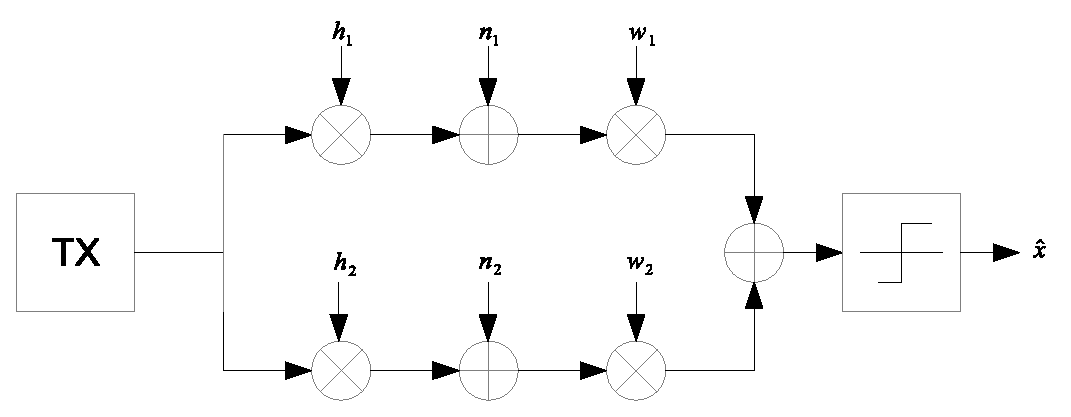
\includegraphics[width=1\textwidth]{MIMO_receiver_2.eps} \\
	&{\sigma_n^2}_1={\sigma_n^2}_2={\sigma_n^2}_1 \\
	&\text{branch SNR: }\bar{\gamma}=\frac{\sigma_x^2}{\sigma_n^2} \\
	&\text{branch 1}\quad\rightarrow\quad\text{Rayleigh}\quad\rightarrow\quad p_\gamma\left(x\right)=\frac{1}{\bar{\gamma}}\mathrm{exp}\left(\frac{x}{\bar{\gamma}}\right) \\
	&\text{branch 2}\quad\rightarrow\quad\text{Nakagami-m}\quad\rightarrow\quad p_\gamma\left(x\right)=\frac{m^mx^{m-1}}{\gamma^{-m}\Gamma\left(m\right)}\mathrm{exp}\left(-\frac{mx}{\bar{\gamma}}\right) \\
	&\text{i.i.d fading}\quad\rightarrow\quad {M_\gamma}_\mathrm{total}\left(s\right)={M_\gamma}_1\left(s\right){M_\gamma}_2\left(s\right) \\
	&\begin{cases}
		\quad\text{first branch}\quad\rightarrow\quad\text{Rayleigh}\quad\rightarrow\quad{M_\gamma}_1\left(s\right)=\left(1-s\bar{\gamma}\right)^{-1} \\
		\quad\text{second branch}\quad\rightarrow\quad\text{Nakagami-m}\quad\rightarrow\quad{M_\gamma}_2\left(s\right)=\left(1-\frac{s\bar{\gamma}}{m}\right)^{-m} \\
	\end{cases} \\
	&\quad\rightarrow\quad{M_\gamma}_\mathrm{total}=\left(1-s\bar{\gamma}\right)^{-1}\left(1-s\frac{\bar{\gamma}}{m}\right)^{-m} \\
	&\text{from lectures notes:} \\
	&\rightarrow\bar{P}_e=\int_0^\infty P_e{p_\gamma}_\mathrm{total}\left(x\right)\mathrm{d}x = \\ 
	&\qquad=\int\limits_0^\infty\frac{1}{\pi}\int\limits_0^{\frac{\left(M-1\right)\pi}{M}}\mathrm{exp}\left(\right)\mathrm{d}\Theta\,{p_\gamma}_\mathrm{total}\left(x\right)\mathrm{d}x= \\
	&\qquad=\frac{1}{\pi}\int\limits_0^{\frac{\left(M-1\right)\pi}{M}}\int\limits_0^\infty\mathrm{exp}\left(\frac{-x\sin^2\left(\frac{\pi}{M}\right)}{\sin^2\Theta}\right){p_\gamma}_\mathrm{total}\left(x\right)\mathrm{d}x\,\mathrm{d}\Theta= \\
	&\qquad=\int\limits_0^\infty e^{sx}{p_\gamma}_\mathrm{total}\left(x\right)\mathrm{d}x={M_\gamma}_\mathrm{total}\left(s\right)
\end{align*}
\begin{align*}
	&\rightarrow\int\limits_0^\infty\mathrm{exp}\left(\frac{-x\sin^2\left(\frac{\pi}{M}\right)}{\sin^2\Theta}\right){p_\gamma}_\mathrm{total}\left(x\right)\mathrm{d}x={M_\gamma}_\mathrm{total}\left(\frac{-\sin^2\left(\frac{\pi}{M}\right)}{\sin^2\Theta}\right) \\
	&\rightarrow\bar{p}_e=\frac{1}{M}\int\limits_0^{\frac{\left(M-1\right)\pi}{M}}{M_\gamma}_\mathrm{total}\left(\frac{-\sin^2\left(\frac{\pi}{M}\right)}{\sin^2\Theta}\right)\mathrm{d}\Theta \\
	&\rightarrow\boxed{\bar{p}_e=\frac{1}{M}\int\limits_0^{\frac{\left(M-1\right)\pi}{M}}\left(1+\frac{\bar{\gamma}\sin^2\left(\frac{\pi}{M}\right)}{\sin^2\Theta}\right)^{-1}\left(1+\frac{\bar{\gamma}\sin^2\left(\frac{\pi}{M}\right)}{m\sin^2\Theta}\right)^{-m}\mathrm{d}\Theta} \\
	&\bar{\gamma}=10\,\mathrm{dB}\qquad M=8\rightarrow 8\mathrm{PSK}\qquad m=3\qquad\Rightarrow\quad\bar{p}_e=0,0476
\end{align*}